\hypersetup{colorlinks}
\usepackage{etoolbox}

%% 
% xelatex tufte fixes 
% https://tex.stackexchange.com/questions/202142/problems-compiling-tufte-title-page-in-xelatex
\renewcommand{\textls}[2][5]{%
  \begingroup\addfontfeatures{LetterSpace=#1}#2\endgroup
}
\renewcommand{\allcapsspacing}[1]{\textls[15]{#1}}
\renewcommand{\smallcapsspacing}[1]{\textls[10]{#1}}
\renewcommand{\allcaps}[1]{\textls[15]{\MakeTextUppercase{#1}}}
\renewcommand{\smallcaps}[1]{\smallcapsspacing{\scshape\MakeTextLowercase{#1}}}
\renewcommand{\textsc}[1]{\smallcapsspacing{\textsmallcaps{#1}}}


%%
% usepackage won't work, already included in docclass?
% paperwidth =  left + width + right                        185
%   width = textwidth (+ marginparsep + marginparwidth)     158
% paperheight = top + height + bottom                       225
%   height = textheight (+ headheight + headsep + footskip) 205
\geometry{
  %showframe,
  twoside,
  includemp,
  includehead,
  includefoot,
  %,
  paperwidth=185mm,
  textwidth=104mm,
  marginparsep=4mm,
  marginparwidth=50mm,
  inner=12mm,
  outer=15mm,
  %,
  paperheight=225mm,
  textheight=195mm,
  headheight=10mm,
  headsep=10mm,
  footskip=0mm,
  top=5mm,
  bottom=15mm
}
%%
% Book metadata
\title{Inside the Game Boy Game Loop}
\author{Wouter Groeneveld}
\publisher{Brain Baking}

%%
% Prints a trailing space in a smart way.
\usepackage{xspace}

% ===================
% = Font/Text Setup =
% ===================
% The fancyvrb package lets us customize the formatting of verbatim
% environments.  We use a slightly smaller font.
\usepackage{fancyvrb}
\fvset{fontsize=\normalsize}

%%
% xelatex-specific font setup - main: mathpazo-style
\usepackage{fontspec}
\setmainfont
     [ BoldFont       = texgyrepagella-bold.otf ,
       ItalicFont     = texgyrepagella-italic.otf ,
       BoldItalicFont = texgyrepagella-bolditalic.otf ]
     {texgyrepagella-regular.otf}
\newfontfamily{\retro}{SuperLegendBoy}[Extension = .ttf]
% for Japanese chars - not needed (yet)
% \usepackage{xeCJK}
% \setCJKmainfont[BoldFont=STHeiti,ItalicFont=STKaiti]{STSong}

% set chapter/section/quote styles to retro font
\usepackage{sectsty}
\partfont{\retro}
\chapterfont{\retro}
\sectionfont{\retro}
\subsectionfont{\retro}
\AtBeginEnvironment{quote}{\retro}

\renewcommand{\labelitemi}{$\circ$}

%%
% styling section/chapter/subsection/...
\usepackage{xcolor}
\definecolor{gb0}{HTML}{19380F}
\definecolor{gb1}{HTML}{306130}
\definecolor{gb2}{HTML}{8BAC12}
\definecolor{gb3}{HTML}{9BBD16}
\usepackage{lipsum}

% 0 = part/chapter nums. 1 = section, 2 = subsection, -1 = disable.
\setcounter{secnumdepth}{0}

% chapter format
\titleformat{\chapter}%
  {\Huge\retro\itshape\color{gb1}}% format applied to label+text
  {\llap{\colorbox{gb0}{\parbox{10.5cm}{\hfill\itshape\Huge\color{white}\thechapter}}}}% label
  {8pt}% horizontal separation between label and title body
  {}% before the title body
  []% after the title body

% set captions of figures to italic
% \setcaptionfont{\itshape}

% ================
% = Images Setup =
% ================
% for png/pdf inclusion (pdfpages: full-page)
\usepackage{graphicx}
\graphicspath{{img/}}
\setkeys{Gin}{width=\linewidth,totalheight=\textheight,keepaspectratio}

% figure caption styles. tufte-book is incompatible with package caption...
% https://tex.stackexchange.com/questions/106416/remove-prefix-from-figure-caption-in-tufte-book-document-class
\makeatletter
\patchcmd{\@caption}
  {\noindent\csname fnum@#1\endcsname: \ignorespaces}
  {}
  {}{}
\makeatother

\newcommand{\marginfig}[4][0cm]{
  \begin{marginfigure}[#1]
    \includegraphics[width=\linewidth]{#2}
    \caption[#4]{#3}
  \end{marginfigure}  
}

\newcommand\cover[4]{
  \begin{marginfigure}[6cm] % assumes \cover is called right after a new chapter.
    \includegraphics[width=\linewidth]{covers/#1.jpg}
    \caption[Cover art for #1]{\textbf{Developer}: #2 \newline \textbf{Release}: #3 \newline \textbf{Genre}: #4}
  \end{marginfigure}  
}

%%
% graphics drawing
\usepackage{tikz}
\usetikzlibrary{shapes.geometric, arrows}

\tikzstyle{startstop} = [rectangle, rounded corners, minimum width=3cm, minimum height=0.7cm,text centered, draw=black]
\tikzstyle{box} = [trapezium, trapezium left angle=70, trapezium right angle=110, minimum width=1cm,  minimum height=0.7cm, text centered, draw=black]
\tikzstyle{arrow} = [thick,->,>=stealth]


%% 
% background test (use \BgThispage on page if 'some' option enabled)
%\usepackage[pages=some]{background}
%\backgroundsetup{
%  scale=1.1,
%  angle=0,
%  opacity=1,  %% adjust
%  contents={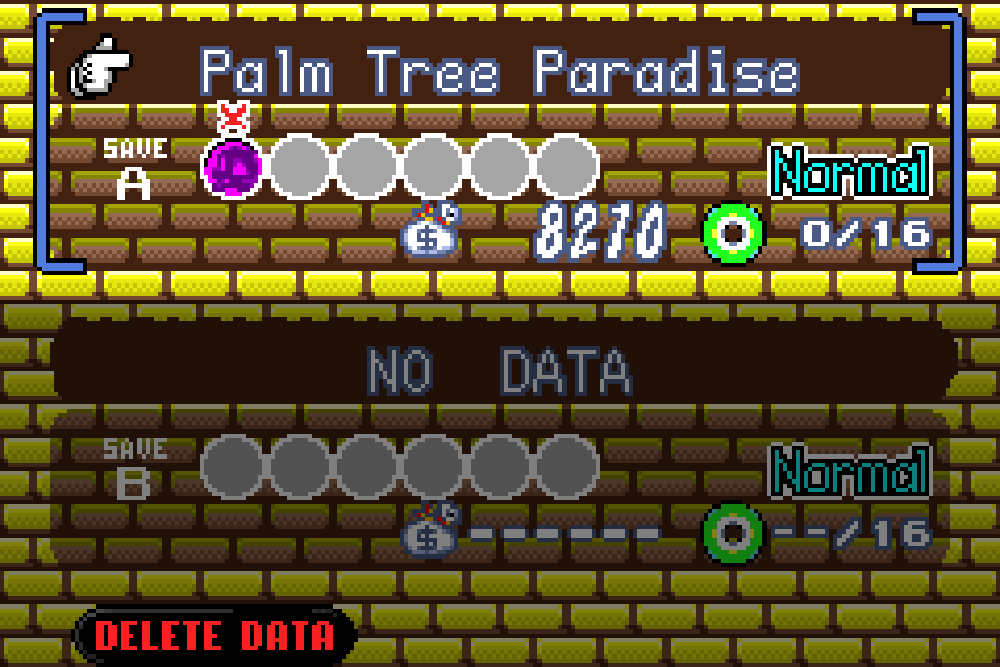
\includegraphics[width=\paperwidth,height=\paperheight]{chapters/wario4.png}}
%}

%% 
% begin new chapter left-side (complications with tufte-book)
%\makeatletter
%\renewcommand*\cleardoublepage{\clearpage\if@twoside
%  \ifodd\c@page \hbox{}\newpage\if@twocolumn\hbox{}%
%  \newpage\fi\fi\fi}
%\makeatother

% Generates the index
\usepackage{makeidx}
\makeindex

%%
% Tufte shortcuts, copied from sample-book.tex
% Prints the month name (e.g., January) and the year (e.g., 2008)
\newcommand{\monthyear}{%
  \ifcase\month\or January\or February\or March\or April\or May\or June\or
  July\or August\or September\or October\or November\or
  December\fi\space\number\year
}

\newenvironment{docspec}{\begin{quotation}\ttfamily\parskip0pt\parindent0pt\ignorespaces}{\end{quotation}}% command specification environment


% Prints an epigraph and speaker in sans serif, all-caps type.
\newcommand{\openepigraph}[2]{%
  %\sffamily\fontsize{14}{16}\selectfont
  \begin{fullwidth}
  \sffamily\large
  \begin{doublespace}
  \noindent\allcaps{#1}\\% epigraph
  \noindent\allcaps{#2}% author
  \end{doublespace}
  \end{fullwidth}
}

